\documentclass[9pt,a4paper]{extarticle}
\usepackage[a4paper,top=1.1cm,bottom=1.0cm,left=1.2cm,right=1.2cm]{geometry}
\usepackage[T1]{fontenc}
\usepackage[utf8]{inputenc}
\usepackage{textcomp}
\usepackage{charter}
\usepackage[scaled=0.86]{helvet}
\usepackage{lmodern}
\usepackage{xcolor}
\usepackage{tikz}
\usepackage{graphicx}
\usepackage{booktabs}
\usepackage{array}
\usepackage{tabularx}
\usetikzlibrary{positioning,arrows.meta,shapes.geometric,backgrounds,fit}

\definecolor{ink}{HTML}{1B2A38}
\definecolor{faint}{HTML}{6E7B87}
\definecolor{rule}{HTML}{C3CCD4}

% Palette lifted from the patient-trend-pulse triage dashboard (src/index.css,
% "Medical Status Colors" / "Vital Sign Colors"), converted from HSL to hex.
\definecolor{ccrit}{HTML}{EF4343}   % --status-red      0 84% 60%
\definecolor{cwarn}{HTML}{E7B008}   % --status-yellow  45 93% 47%
\definecolor{csafe}{HTML}{16A249}   % --status-green  142 76% 36%
\definecolor{carte}{HTML}{F97415}   % --status-orange  25 95% 53%
\definecolor{cunev}{HTML}{94A3B8}   % --muted-foreground

\setlength{\parindent}{0pt}
\pagestyle{empty}

\newcommand{\hdr}[2][]{%
  {\sffamily\bfseries\footnotesize\color{ink}\MakeUppercase{#2}}%
  {\sffamily\footnotesize\color{faint}\,#1}%
  \par\vspace{1pt}{\color{rule}\hrule height .6pt}\vspace{3pt}}
% The patient's own words get a bigger header than the model's sections. On a card whose
% other content is machine output, the transcript is the only evidence that came from the
% patient, and it was previously the smallest thing on the page.
\newcommand{\hdrbig}[2][]{%
  {\sffamily\bfseries\normalsize\color{ink}\MakeUppercase{#2}}%
  {\sffamily\small\color{faint}\,#1}%
  \par\vspace{2pt}{\color{rule}\hrule height .8pt}\vspace{4pt}}
\newcommand{\Q}{{\bfseries\normalsize ?}}

% --- anatomy pins. \pinXXXX puts the number on the point; \leadXXXX draws a leader.
\newcommand{\pinbase}[5]{\filldraw[#4,draw=white,line width=.5pt] (#2,#3) circle (1.85mm)
  node[#5,font=\bfseries\sffamily\fontsize{5}{5}\selectfont] {#1};}
\newcommand{\pincrit}[3]{\pinbase{#1}{#2}{#3}{ccrit}{white}}
\newcommand{\pinwarn}[3]{\pinbase{#1}{#2}{#3}{cwarn}{ink}}
\newcommand{\pinsafe}[3]{\pinbase{#1}{#2}{#3}{csafe}{white}}
\newcommand{\pinarte}[3]{\pinbase{#1}{#2}{#3}{carte}{white}}
\newcommand{\pinunev}[3]{\filldraw[white,draw=cunev,line width=.6pt] (#2,#3) circle (1.75mm)
  node[cunev,font=\bfseries\sffamily\fontsize{5}{5}\selectfont] {#1};}
\newcommand{\leadbase}[6]{\draw[#6,line width=.4pt] (#2,#3) -- (#4,#5);
  \filldraw[#6] (#2,#3) circle (0.45mm);}
\newcommand{\leadcrit}[5]{\leadbase{#1}{#2}{#3}{#4}{#5}{ccrit}\pincrit{#1}{#4}{#5}}
\newcommand{\leadwarn}[5]{\leadbase{#1}{#2}{#3}{#4}{#5}{cwarn}\pinwarn{#1}{#4}{#5}}
\newcommand{\leadsafe}[5]{\leadbase{#1}{#2}{#3}{#4}{#5}{csafe}\pinsafe{#1}{#4}{#5}}
\newcommand{\leadarte}[5]{\leadbase{#1}{#2}{#3}{#4}{#5}{carte}\pinarte{#1}{#4}{#5}}
\newcommand{\leadunev}[5]{\leadbase{#1}{#2}{#3}{#4}{#5}{cunev}\pinunev{#1}{#4}{#5}}

\begin{document}

%================================================================ header
{\sffamily\bfseries\large\color{ink} KOVALENKO, 34, M}\hfill
{\sffamily\small\color{faint} 2026-08-29 14:32 \;\textperiodcentered\; Stab.\ point \textit{Sokil}}\\[2pt]
{\color{ink}\hrule height 1pt}
\vspace{5pt}

%================================================================ transcript (first)
\hdrbig[--- verbatim, no clinician inference]{What the patient said}
\small
\setlength{\extrarowheight}{2.5pt}
\begin{tabularx}{\linewidth}{@{}l l X l@{}}
\toprule
\textbf{Point} & \textbf{Time} & \textbf{Said} & \textbf{Requests}\\
\midrule
POI            & 11:05 & ``head hurts, can't see right''    & water\\
CCP            & 12:40 & neck pain turning left             & water $\times2$\\
Stab.\ Sokil   & 14:20 & \textbf{headache worse lying flat} & asks about brother $\times2$\\
\bottomrule
\end{tabularx}
\setlength{\extrarowheight}{0pt}
\vspace{4pt}

{\footnotesize\color{ink}\textbf{Note.} ``Worse lying flat'' is positional and is evidence about
intracranial pressure that the model did not produce. It arrives from the patient and is not
reconciled with the model output below --- where the two disagree, both are shown.}

\vspace{7pt}

%================================================================ vitals + input
\noindent\begin{minipage}[t]{0.485\textwidth}
\hdr[{\color{ccrit}(14:28 --- 4 min old)}]{Vitals}
\footnotesize
\begin{tabularx}{\linewidth}{@{}lX@{}}
BP        & 104/62\quad(MAP 76)\\
HR        & 118\\
SpO$_2$   & 94\% RA\\
RR        & 24\\
GCS       & 14\quad(E4 V4 M6)\\
Temp      & 36.4\,\textcelsius\\
Cap refill& 3\,s\\
\end{tabularx}
\end{minipage}\hfill
\begin{minipage}[t]{0.485\textwidth}
\hdr{Model input}
\footnotesize
\begin{tabularx}{\linewidth}{@{}lX@{}}
Recording   & 081, 100\,Hz ICP + ABP\\
Manoeuvre   & jugular compression, 118\,s\\
Window      & $-120$ to $+268$\,s\\
Fit         & RMSE 0.31\,mmHg / 261 beats\\
Identifiable& 13 of 16 windows\\
\end{tabularx}
\vspace{2pt}
{\scriptsize\color{faint}RMSE is the typical gap between the model's ICP and the measured
ICP. 0.31\,mmHg is small; it means the model reproduces the pressure, not that the parts
below are right.\par}
\end{minipage}

\vspace{9pt}

%================================================================ title above the picture
{\sffamily\bfseries\LARGE\color{ink} PULSATION ANALYSIS}\hfill
{\sffamily\footnotesize\color{faint} the CSF and venous circuit as 9 compartments and
12 interfaces \;\textperiodcentered\; colour = status, number = key below}\\[3pt]
{\color{ink}\hrule height 1.1pt}
\vspace{4pt}

\centering
\begin{tikzpicture}
  \node[anchor=south west,inner sep=0] (img)
    {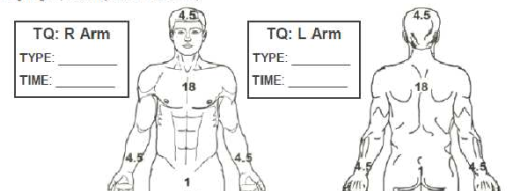
\includegraphics[width=0.92\textwidth]{../figures/body_template_upper.png}};
  \begin{scope}[x={(img.south east)},y={(img.north west)}]
    \fill[white] (0.0078,0.49875) rectangle (0.24951,0.9269);
    \fill[white] (0.46004,0.49875) rectangle (0.69396,0.9269);
    \fill[white,opacity=0.5] (0,0) rectangle (1,1);
    \leadwarn{1}{0.34698}{0.84336}{0.2729}{0.91646}
    \leadcrit{2}{0.36842}{0.81203}{0.2729}{0.82769}
    \leadunev{3}{0.38986}{0.80159}{0.44444}{0.84336}
    \leadunev{4}{0.34308}{0.77548}{0.2729}{0.73893}
    \leadunev{5}{0.36257}{0.75459}{0.44444}{0.75982}
    \leadunev{6}{0.39181}{0.8538}{0.44444}{0.9269}
    \leadunev{7}{0.36842}{0.71805}{0.2729}{0.65017}
    \leadunev{8}{0.35088}{0.70238}{0.2729}{0.5614}
    \leadunev{9}{0.34503}{0.6815}{0.2729}{0.47264}
    \leadarte{10}{0.33918}{0.65017}{0.2729}{0.38388}
    \pinunev{11}{0.37817}{0.50397}
    \pinsafe{12}{0.82456}{0.9269}
    \pincrit{13}{0.80117}{0.89035}
    \pinarte{14}{0.84016}{0.71282}
    \pinunev{15}{0.84211}{0.45698}
    \pincrit{16}{0.82456}{0.40998}
    \pinunev{17}{0.79727}{0.49353}
    \pinunev{18}{0.80117}{0.33166}
    \pincrit{19}{0.82456}{0.21679}
    \pinunev{20}{0.846}{0.30033}
    \pinunev{21}{0.85965}{0.16458}
  \end{scope}
\end{tikzpicture}

\vspace{3pt}
{\footnotesize\color{ink}%
\tikz[baseline=-.5ex]\filldraw[ccrit] (0,0) circle (1.5mm); warning \quad
\tikz[baseline=-.5ex]\filldraw[cwarn] (0,0) circle (1.5mm); borderline \quad
\tikz[baseline=-.5ex]\filldraw[csafe] (0,0) circle (1.5mm); within ref. \quad
\tikz[baseline=-.5ex]\filldraw[carte] (0,0) circle (1.5mm); artefact \quad
\tikz[baseline=-.5ex]\filldraw[white,draw=cunev,line width=.6pt] (0,0) circle (1.4mm); \Q\ not evaluated\par}

\vspace{7pt}
\raggedright
\hdr[--- four terms on this card that do not mean what they usually mean]{How to read this}
\footnotesize
\noindent\begin{minipage}[t]{0.485\textwidth}
\begin{tabularx}{\linewidth}{@{}p{1.35cm}X@{}}
\textbf{w\,0.63} & how far \emph{outside} the normal band that part sits. 0 = at the edge of
normal, 1.0 = at the danger bound, higher = further out. It is \textbf{not} a probability and
\textbf{not} a severity score.\\[3pt]
\Q & nothing on this card measured that part. It means \textbf{not measured}. It does
\textbf{not} mean normal --- 13 of the 21 parts are like this.\\
\end{tabularx}
\end{minipage}\hfill
\begin{minipage}[t]{0.485\textwidth}
\begin{tabularx}{\linewidth}{@{}p{1.35cm}X@{}}
{\color{carte}\textbf{artefact}} & the model bent this number to make its own arithmetic
work. It is a statement about the model, \textbf{not about this patient}. Do not read the
value.\\[3pt]
\textbf{the dots} & lumped parts of the CSF and venous circuit, drawn where that region
roughly is. They are \textbf{not surgical landmarks}.\\
\end{tabularx}
\end{minipage}

\vspace{3pt}
{\footnotesize\color{ink}\textbf{Where the numbers come from.} A two-minute jugular
compression, held by hand. Before it starts almost nothing here can be measured at all; the
compression is what makes the venous numbers estimable, and \textbf{Identifiable} above counts
the windows where that worked. Where it did not, the value is a guess and is marked \Q.\par}

\vspace{6pt}
\hdr{Component key}
{\scriptsize
\begin{tabular}{@{}r@{~}l l@{}}
    {\color{cwarn}$\bullet$}~1 & Cerebral arterial & {\scriptsize w\,0.39} \\
    {\color{ccrit}$\bullet$}~2 & Intracranial CSF & {\scriptsize \textbf{w\,0.63}} \\
    {\color{cunev}$\bullet$}~3 & Cerebral venous & {\scriptsize \Q} \\
    {\color{cunev}$\bullet$}~4 & Arteriolar bed & {\scriptsize \Q} \\
    {\color{cunev}$\bullet$}~5 & Capillary bed & {\scriptsize \Q} \\
    {\color{cunev}$\bullet$}~6 & Cerebral venous outflow & {\scriptsize \Q} \\
    {\color{cunev}$\bullet$}~7 & Craniospinal CSF channel & {\scriptsize \Q}\\
\end{tabular} \hfill
\begin{tabular}{@{}r@{~}l l@{}}
    {\color{cunev}$\bullet$}~8 & Sinus to jugular bulb & {\scriptsize \Q} \\
    {\color{cunev}$\bullet$}~9 & Jugular bulb & {\scriptsize \Q} \\
    {\color{carte}$\bullet$}~10 & Internal jugular & {\scriptsize \textbf{ARTEFACT}} \\
    {\color{cunev}$\bullet$}~11 & Systemic venous & {\scriptsize \Q} \\
    {\color{csafe}$\bullet$}~12 & Dural sinus & {\scriptsize w\,0.11} \\
    {\color{ccrit}$\bullet$}~13 & CSF absorption, cranial & {\scriptsize \textbf{w\,1.53}} \\
    {\color{carte}$\bullet$}~14 & Vertebral collateral & {\scriptsize \textbf{ARTEFACT}}\\
\end{tabular} \hfill
\begin{tabular}{@{}r@{~}l l@{}}
    {\color{cunev}$\bullet$}~15 & Vertebral plexus & {\scriptsize \Q} \\
    {\color{ccrit}$\bullet$}~16 & Spinal dural sac & {\scriptsize \textbf{w\,0.63}} \\
    {\color{cunev}$\bullet$}~17 & Azygos return & {\scriptsize \Q} \\
    {\color{cunev}$\bullet$}~18 & Paravertebral & {\scriptsize \Q} \\
    {\color{ccrit}$\bullet$}~19 & CSF absorption, spinal & {\scriptsize \textbf{w\,1.53}} \\
    {\color{cunev}$\bullet$}~20 & Plexus drainage & {\scriptsize \Q} \\
    {\color{cunev}$\bullet$}~21 & Plexus shunt & {\scriptsize \Q}\\
\end{tabular}
\par}
\vspace{3pt}
{\scriptsize\color{faint}\textbf{13 of 21} components carry \Q: no streamed parameter governs
them. \Q\ means \textbf{not estimated}, never \textbf{normal}. The two \textbf{artefact}
components are rulebook \textbf{R1} (tube-law escape) --- the fit inflated the resting jugular
to 6.12\,cm\textsuperscript{2} against a physiological 0.8--2.0 and blocked the collateral to
manufacture the measured ICP step. Neither is a statement about this patient.}

\vspace{5pt}
{\color{rule}\hrule height .6pt}
\vspace{3pt}
{\scriptsize\color{faint}
\textbf{Provenance.} Component weights, values and the R1 determination are \textbf{real
output} for recording 081, final window ($t_\mathrm{end}=268.4$\,s).
Name, age, sex, vitals, evacuation points and transcript are \textbf{synthetic} --- the dataset
contains none of these.
\textbf{Weight} is the excursion beyond the healthy band (1.0 at the pathological bound),
discounted by identifiability; it is not a probability.
\textbf{No healthy controls exist in this dataset} --- every bound is from literature.
The underlying model overestimates ICP pulse amplitude under compression by ${\sim}7\times$
from a diagnosed cause, which is why the jugular carries a QC bound rather than a clinical one.
Pin positions are schematic --- the anatomical region a lumped element stands for, not a
surgical landmark. Not a diagnosis. Confirm before acting.}

\end{document}
